% id: 0341
% book: RPM 중3-2 수학 · 03 원과 직선
% section: 중단원 마무리하기
% figure: crop:fig-0341.png
% answer: ②
% answer_source: 답지
% variant_level: 0 (원본 전사)
% 이 파일은 build.mjs 가 items.json 에서 만든다. 고칠 때는 items.json 을 고친다.
\noindent\begin{minipage}[t]{0.58\linewidth}\vspace{0pt}\raggedright 오른쪽 그림과 같이 반지름의 길이가 $6\mkern3mu \mathrm{cm}$인 원~$\pt{O}$에서 점~$\pt{T}$는 원~$\pt{O}$의 접점이고 $\angle\pt{POT}=60^\circ$일 때, 색칠한 부분의 넓이는?\end{minipage}\hfill\begin{minipage}[t]{0.4\linewidth}\vspace{0pt}\centering \setlength{\dmfigw}{92.6pt}\ifdim\dmfigw>\linewidth\setlength{\dmfigw}{\linewidth}\fi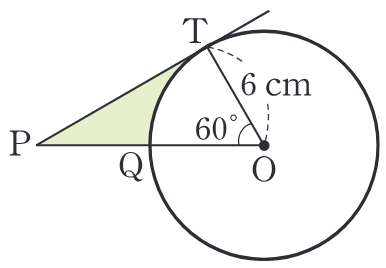
\includegraphics[width=\dmfigw]{figures/fig-0341.png}\end{minipage}\par
\begin{choicesv}{$(18\sqrt{3}-8\pi)\mkern3mu \mathrm{cm}^2$}{$(18\sqrt{3}-6\pi)\mkern3mu \mathrm{cm}^2$}{$(36\sqrt{3}-12\pi)\mkern3mu \mathrm{cm}^2$}{$(36\sqrt{3}-8\pi)\mkern3mu \mathrm{cm}^2$}{$(36\sqrt{3}-6\pi)\mkern3mu \mathrm{cm}^2$}\end{choicesv}
